\documentclass[a4paper,10pt]{article}
\usepackage[utf8]{inputenc}
\usepackage{cite}
\usepackage{amsmath,amssymb,amsfonts}
\usepackage{algorithmic}
\usepackage{float}
\usepackage{hyperref}
\usepackage{graphicx}
\usepackage{textcomp}
\usepackage{listings}
\usepackage{epsfig}
\usepackage{tikz}
\usepackage{pgfplots}

\pgfplotsset{compat=1.15}

\providecommand{\keywords}[1]{{\bf{\em Index terms---}} #1}
\newfloat{program}{thp}{lop}
\floatname{program}{Listing}
\title{Title}
\date{}
\author{Martino Ferrari \and Giordano Ferrari}

\begin{document}
\maketitle
\begin{abstract}

Lorem {\bf ipsum}
dolor sit amet, consectetuer adipiscing elit, sed diam nonummy nibh euismod tincidunt ut
laoreet dolore magna aliquam erat volutpat. Ut wisi enim ad minim veniam, quis nostrud exerci tation
ullamcorper suscipit lobortis nisl ut aliquip ex ea commodo consequat. Duis autem vel eum iriure dolor in hendrerit in
vulputate velit esse molestie consequat, vel illum dolore eu feugiat nulla facilisis at vero eros et
accumsan et iusto odio dignissim qui blandit praesent luptatum zzril delenit augue duis dolore te feugait nulla facilisi.
Nam liber tempor cum soluta nobis eleifend option congue nihil imperdiet doming id quod mazim placerat facer possim assum.

\keywords{Semantic, Web, Markdown}
\end{abstract}

\tableofcontents
\section{Chapter}

Lorem ipsum
dolor sit amet, consectetuer adipiscing elit, sed diam nonummy nibh euismod tincidunt ut
laoreet dolore magna aliquam erat volutpat. Ut wisi enim ad minim veniam, quis nostrud exerci tation
laoreet dolore magna aliquam erat volutpat. Ut wisi enim ad minim veniam, quis nostrud exerci tation
ullamcorper suscipit lobortis nisl ut aliquip ex ea commodo consequat. Duis autem vel eum iriure dolor in hendrerit in
vulputate velit esse molestie consequat, vel illum dolore eu feugiat nulla facilisis at vero eros et
ullamcorper suscipit lobortis nisl ut aliquip ex ea commodo consequat. Duis autem vel eum iriure dolor in hendrerit in
vulputate velit esse molestie consequat, vel illum dolore eu feugiat nulla facilisis at vero eros et

\begin{table}
\begin{center}

\begin{tabular}{ | l | c | r | }
\hline
{\bf Col. 1} & {\bf Col.2} & {\bf Col. 3}\\
\hline
A & B & C\\
D & E & F\\
G & H & I\\
\hline
\end{tabular}

\caption{This is a table.}
\label{tab:simple}
\end{center}
\end{table}

accumsan et iusto odio dignissim qui blandit praesent luptatum zzril delenit augue duis dolore te feugait nulla facilisi.
Nam liber tempor cum soluta nobis eleifend option congue nihil imperdiet doming id quod mazim placerat facer possim assum.
laoreet dolore magna aliquam erat volutpat. Ut wisi enim ad minim veniam, quis nostrud exerci tation
ullamcorper suscipit lobortis nisl ut aliquip ex ea commodo consequat. Duis autem vel eum iriure dolor in hendrerit in
vulputate velit esse molestie consequat, vel illum dolore eu feugiat nulla facilisis at vero eros et


\subsection{Section}

Lorem ipsum
dolor sit amet, consectetuer adipiscing elit, sed diam nonummy nibh euismod tincidunt ut
laoreet dolore magna aliquam erat volutpat. Ut wisi enim ad minim veniam, quis nostrud exerci tation this is a reference to the figure (\ref{fig:falcon}) representing a falcon rocket.

\begin{program}
\begin{center}

\begin{lstlisting}[language=c]
int main(int argc, char** argv)
{
    printf("hello world!\n");
    return 0;
}
\end{lstlisting}

\caption{This is a simple code.}
\end{center}
\end{program}

ullamcorper suscipit lobortis nisl ut aliquip ex ea commodo consequat. Duis autem vel eum iriure dolor in hendrerit in
vulputate velit esse molestie consequat, vel illum dolore eu feugiat nulla facilisis at vero eros et
accumsan et iusto odio dignissim qui blandit praesent luptatum zzril delenit augue duis dolore te feugait nulla facilisi.
Nam liber tempor cum soluta nobis eleifend option congue nihil imperdiet doming id quod mazim placerat facer possim assum.
This is a link \href{www.google.com"}{google}


\subsubsection{Subsection}

This is a reference \cite{fnref:1}.


This is an inline formula \(x+3 = 2^2\) while this one is a block formula


\[
x = \sum_{i=-10}^n e^{-|n|}
\]


The following instead is a numbered and labeled equation:

\begin{equation}
\label{eq:1}
x = \sum_{i=-10}^n e^{-|n|}
\end{equation}
The reference to a floating element is done in this way: the equation (\ref{eq:1}) show absolutely nothing.
mcorper suscipit lobortis nisl ut aliquip ex ea commodo consequat. Duis autem vel eum iriure dolor in hendrerit in
vulputate velit esse molestie consequat, vel illum dolore eu feugiat nulla facilisis at vero eros et
accumsan et iusto odio dignissim qui blandit praesent luptatum zzril delenit augue duis dolore te feugait nulla facilis


\subsubsection{Another subsection}

This a plot

\begin{figure}
\begin{center}

\begin{lstlisting}[language=charter]
width: 400
height: 300
plot:
    x: range: 0 2 20
    y: math: exp(-(x^2))
    label: gauss
x-axis:
    label: frequency
y-axis:
    label: energy
\end{lstlisting}

\caption{This is a simple plot, with linear axis and {\bf no} title.}
\label{fig:plot}
\end{center}
\end{figure}

\subsection{Second section}

Lorem ipsum
dolor sit amet, consectetuer adipiscing elit, sed diam nonummy nibh euismod tincidunt ut
laoreet dolore magna aliquam erat volutpat. Ut wisi enim ad minim veniam, quis nostrud exerci tation
ullamcorper suscipit lobortis nisl ut aliquip ex ea commodo consequat. Duis autem vel eum iriure dolor in hendrerit in

\begin{figure}
\begin{center}

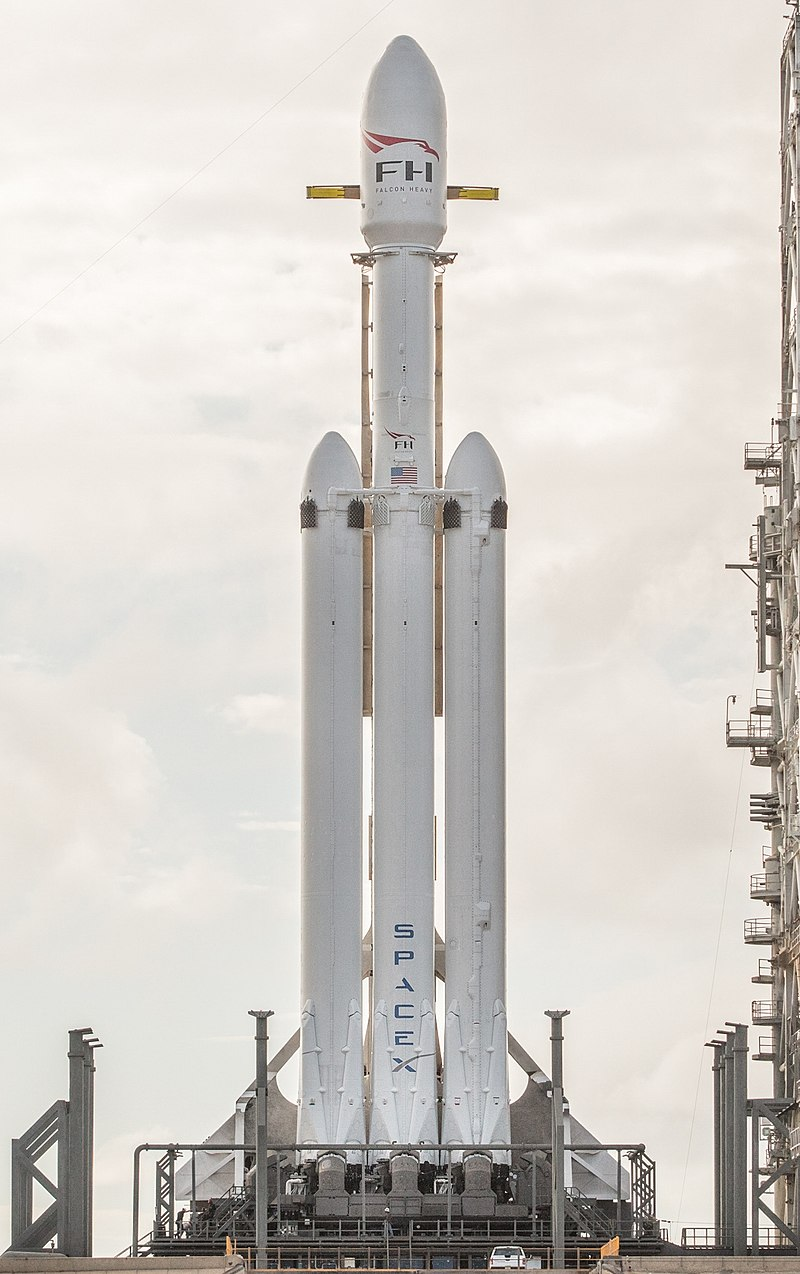
\includegraphics[width=\linewidth]{Falcon_Heavy.jpg}

\caption{This is an image.}
\label{fig:falcon}
\end{center}
\end{figure}

vulputate velit esse molestie consequat, vel illum dolore eu feugiat nulla facilisis at vero eros et
accumsan et iusto odio dignissim qui blandit praesent luptatum zzril delenit augue duis dolore te feugait nulla facilisi.
Nam liber tempor cum soluta nobis eleifend option congue nihil imperdiet doming id quod mazim placerat facer possim assum.


\begin{thebibliography}{00}
\bibitem{fnref:1}This is a reference.


\end{thebibliography}
\end{document}
